
\chapter{Localization of orbit distortion}
\label{sec:localisation}

Correcting the orbit is costly and has never a perfect result. Instead of dealing with the effects, we can deal with the sources of the distortions. If none is really obvious (\textit{eg.} a non-isolated transformer, the 50~Hz perturbation of the main power), the orbit can give us some hints.

We call kick the place where the orbit brutally changes its angle as shown in Fig.~\ref{fig:kick}.

\begin{figure}[!h]
	\centering
	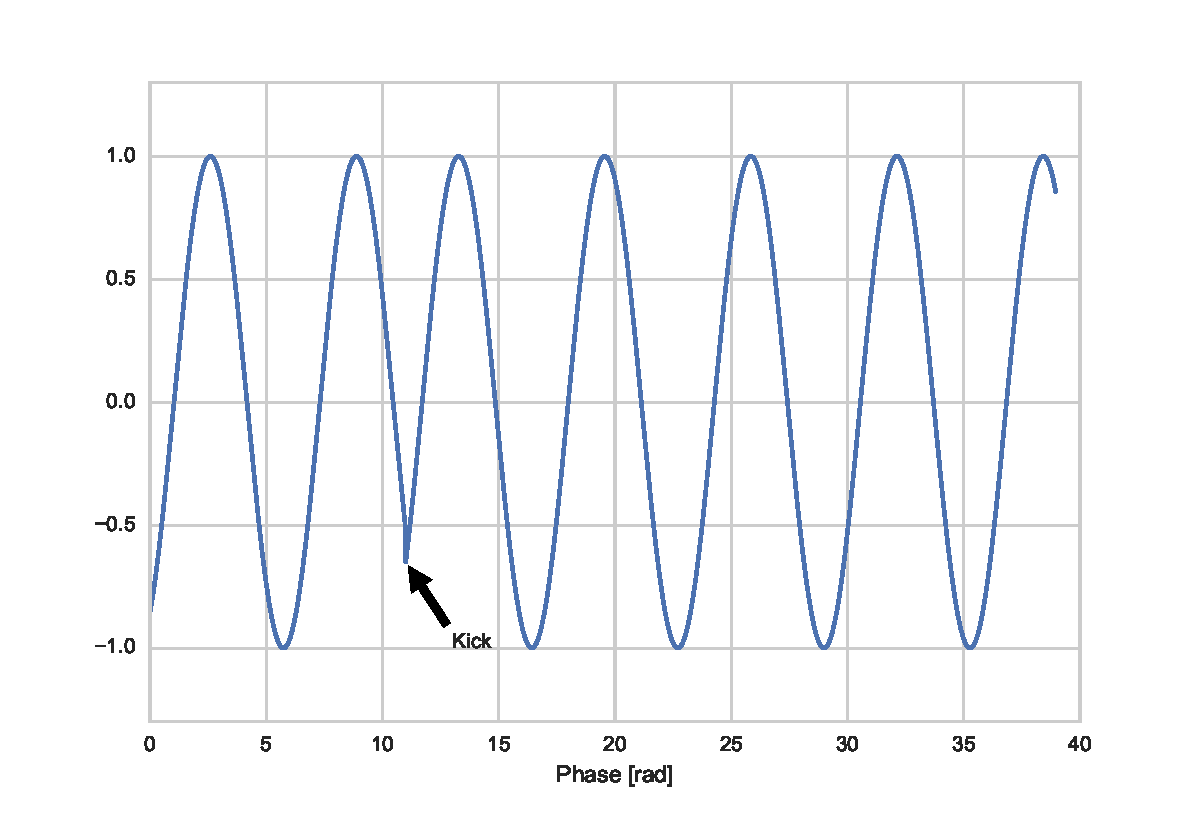
\includegraphics[width=.9\linewidth]{img/kick}
	\caption{\label{fig:kick}Example of kick in the orbit}
\end{figure}

\section{Theory}
\label{ssec:loc_theory}

\subsection{Theoretical setting of the problem}

Everything is described here with the phase variable $\phi = \int\limits_{0}^s \frac{d\sigma}{\beta(\sigma)}$. The spatial variable is only used to have a connection between the result and the actual ring. The explanation will be led with the $x$ variable, but is also valid with the $y$ one.

Let one kick be at $\phi = \hat{\phi}$. The orbit is modified and oscillates with a constant period of $2 \pi$. Because there is {\em only one} kick and according to the closed orbit condition, the oscillation after the kick will be stable for one revolution. Furthermore, the orbit must be continuous on all points, thus at the kick position too.

Let's consider two revolutions, in order to be sure to find one full revolution without kick. Let $\phi_\mathrm{ext} \in [0, 4 \pi Q]$ be this new phase (\textit{ext} for extended). The phase $\phi_0$ where the kick happens is the one so that 
\begin{equation}
\exists (b, c) \in \mathbb{R}^2:
\forall \phi \in [\phi_0, \phi_0 + 2 \pi Q], \quad
x(\phi) = b \sin(\phi + c)
\end{equation}

We have a problem with 3 unknowns to determine: $\phi_0, b, c$. 

\subsection{Practical setting}

We have $m$ BPMs only, distributed around the orbit.
Therefore we define:
\begin{align}
\begin{cases}
\vec{\phi} = [\phi_0, \phi_1, ..., \phi_{m-1}] \\
\vec{x} = [x_0, x_1, ..., x_{m-1}]
\end{cases} \quad \mathrm{and} \quad
\begin{cases}
\vec{\phi}_\mathrm{ext} = [\vec{\phi}, \vec{\phi}+2\pi Q ]\\
\vec{x}_\mathrm{ext} = [\vec{x}, \vec{x}]
\end{cases}
\end{align}

\subsection{Solving the problem}

To find the kick in the orbit it suffices to find a sine that fits in $\vec{x}_\mathrm{ext}$.

An algorithm is designed to find a sine over a revolution, beginning at each BPM and keep the one that fit at best:
\begin{align}
\forall k \in &[0, m-1], \nonumber \\
&\begin{cases}
\vec{\phi}^k = [\vec{\phi}_\mathrm{ext}(k), \vec{\phi}_\mathrm{ext}(k+1), \cdots,  \vec{\phi}_\mathrm{ext}(k+m-1)]\\
\vec{x}^k = [\vec{x}_\mathrm{ext}(k), \vec{x}_\mathrm{ext}(k+1), \cdots,  \vec{x}_\mathrm{ext}(k+m-1)]\\
\tilde{\vec{x}} = \mathtt{fit\_sine}(\vec{x}^k, \vec{\phi}^k)
\end{cases}
\end{align}

It is then defined

\begin{equation}
k_0 = \underset{k \in [0, m-1]}{\textrm{argmin}}\{||\tilde{\vec{x}}-\vec{x}^k||_2\}
\end{equation}

The kick is between $\phi_{k_0-1}$ and $\phi_{k_0+1}$, and we assume that the closest sine is $\tilde{x}(\phi) = b \sin(\phi + c) $.

To find the exact position of the kick, we use the property of closed orbit: the orbit must be continuous also at the kick phase, which means that $\hat{\phi}$ is the solution of
\begin{equation}
b \sin(\phi + c) = b\sin(\phi+c-2 \pi Q), \qquad \mathrm{with}~ \phi \in [\phi_{k_0-1}, \phi_{k_0+1}]
\end{equation}
or, with the numerical approach, 
\begin{equation}
\hat{\phi} =  \underset{\phi \in [\phi_{k_0-1}, \phi_{k_0+1}]}{\textrm{argmin}}\{|b \sin(\phi + c) - b\sin(\phi+c-2 \pi Q)|\}
\end{equation}

\remark For this last step, we use a \textit{linspace} between $\phi_{k_0-1}$ and $\phi_{k_0+1}$ with more than 1000 points.

\remark One should be careful if $k_0 = 0$ (resp. $k_0 = m-1$) and set $\phi_{k_0-1} =\phi_{m-1}$ (resp. $\phi_{k_0+1} = \phi_{0}$). 

\subsection{Finding the good sine}
Several methods are possible to find the best matching sine, for example by using:
\begin{itemize}
	\item a pseudo-inversion
	\item a scalar-product with a sine (resp. a cosine)
\end{itemize}

\paragraph{Pseudo-inversion}
The problem can be set as a linear equation problem as follow.
\begin{align}
&\forall k \in [0,m-1], \tilde{x}(\phi_k) = a_1 \cos(\phi_k) + a_2 \sin(\phi_k) + a \nonumber \\
%
\implies &
\begin{pmatrix}
1 & \cos(\phi_0) & \sin(\phi_0) \\
1 & \cos(\phi_1) & \sin(\phi_1) \\
\vdots & \vdots & \vdots \\
1 & \cos(\phi_{m-1}) & \sin(\phi_{m-1}) \\
\end{pmatrix}
\begin{pmatrix}
a \\ a_1 \\ a_2
\end{pmatrix}
=
\begin{pmatrix}
x_0 \\ x_2 \\ \vdots \\ x_{m-1}
\end{pmatrix} \nonumber
\\
%
\implies &
\begin{pmatrix}
a \\ a_1 \\ a_2
\end{pmatrix}
= 
\mathrm{pseudo\_inv}
\begin{pmatrix}
1 & \cos(\phi_0) & \sin(\phi_0) \\
1 & \cos(\phi_1) & \sin(\phi_1) \\
\vdots & \vdots & \vdots \\
1 & \cos(\phi_{m-1}) & \sin(\phi_{m-1}) \\
\end{pmatrix}
\begin{pmatrix}
x_0 \\ x_2 \\ \vdots \\ x_{m-1}
\end{pmatrix}
\end{align}

The pseudo inverse is calculated in \texttt{Matlab} with \verb$a = M\x$ and in \texttt{python} with \verb$a = numpy.linalg.lstsq(M, x)$ (least-squares solution).

\paragraph{Scalar product with a sine (resp. cosine)}
Since the orbit is expected to be written as
\begin{equation*}
x(\phi) = a_1 \cos(\phi) + a_2 \sin(\phi) + a
\end{equation*}
we can also describe it as
\begin{equation}
x(\phi) = \scal{x}{\cos} \cos(\phi) + \scal{x}{\sin} \sin(\phi) + \scal{x}{1}
\end{equation}
with $\scal{f}{g}$ being the scalar product for real functions: $\int_T f(t)g(u)dt$.

In our numerical case, we approximate this scalar product by its vectorial counterpart by:

\begin{align*}
\scal{\vec{f}}{\vec{g}}: \quad
 &\mathcal{R}^n \times \mathcal{R}^n \longrightarrow \mathcal{R} \\
 & (\vec{f},\vec{g}) \quad\longmapsto \quad \frac{1}{n}\sum\limits_{k=0}^{n-1} f_i g_i
\end{align*}

\paragraph{Coefficient format}
By defining $b = \sqrt{a_1^2+a_2^2}$ and $c = \mathrm{atan2}(a_1, a_2)$  we can write

\begin{equation*}
\tilde{x}(\phi) = a + a_1 \cos(\phi) + a_2 \sin(\phi) = a + b \sin(\phi + c).
\end{equation*} 

\section{Applications}
\todo[inline]{NOT UPDATED: DO NOT CORRECT THIS}
\subsection{Getting the position of a perturbation at a given frequency}
In this section, we deal with a perturbation at a given frequency $f$. The training data is the time signal of all BPMs.

As the perturbation has a known frequency, we extract its complex amplitude from the signal of each BPM with a Fourier transform:

\begin{equation}
\forall i \in [1, \mathrm{BPM\_nb}], \qquad 
\begin{cases}
\vec{X}_i = \mathrm{FFT}(\vec{x}_i) \\
c_i = \vec{X}_i(f)
\end{cases}
\end{equation}

\paragraph{Case of a unique perturbation source}

If the perturbation is unique, then all complex amplitude exactly describe the same sine of frequency $f$ and phase $\alpha_0$. It allows us to describe the complex vector $\vec{c}$ with $\vec{\hat{c}}$, which is real.

\begin{align}
&\alpha_0 = \underset{\alpha \in [0, 2\pi]}{\textrm{argmin}}\{\mathcal{R}e (\vec{c} \cdot e^{-j\alpha}) \} \\
&\vec{\hat{c}} = \mathcal{I}m (\vec{c} \cdot e^{-j\alpha_0})
\end{align}

The new signal $\vec{\hat{c}}$ can be used as an orbit signal: we have one orbit amplitude for each BPM: the kick can be extracted from it with the previous method described in Section \ref{ssec:loc_theory}.


\paragraph{Case of several perturbation sources}
If there are several perturbation sources, a $\alpha_0$ that let the cosine part vanish cannot be found. 


\section{Implementation}
\begin{python}[caption=Get the kick]
	import matplotlib.plt as plt
	import search_kick.core as skcore
	
	# Dataset
	orbit = ..
	phase = ..
	tune = ..
	
	# Get the kick and rebuild the ideal sine
	kick_phase, sin_coef = skcore.get_kick(orbit, phase, tune)
	sine, phase_th = skcore.build_sine(kick_phase, tune, sin_coef)
	
	# Plot the results
	plt.plot(phase, orbit, '-b')
	plt.plot(phase_th, sine, '-g')
	plt.axvline(kick, -2, 2)	
\end{python}


\section{Examples}

